% !TeX program = xelatex
\documentclass[9pt]{beamer}
\usepackage{xcolor}
\definecolor{orange}{HTML}{F67941}
\definecolor{red}{HTML}{AC454A}
\definecolor{brown}{HTML}{EAD296}
\definecolor{darkgrey}{HTML}{313630}
\usefonttheme{professionalfonts} % using non standard fonts for beamer
\usefonttheme{serif} % default family is serif
\usepackage{fontspec}
\usepackage{natbib}
%\usepackage[T1]{fontenc}

\bibliographystyle{abbrv}
%\setmainfont{Liberation Serif}
%\setmainfont{Liberation Serif}
\setmainfont{Comfortaa}
%\usepackage[T1]{fontenc}

\setbeamercolor{frametitle}{bg=orange,fg=white}
\setbeamercolor{author in head/foot}{bg=orange,fg=white}



%\setbeamertemplate{itemize items}[circle]
\useinnertheme{circles}
\setbeamercolor{palette primary}{bg=orange,fg=white}
%\setbeamercolor{palette secondary}{bg=red,fg=white}
\setbeamertemplate{itemize item}{\color{darkgrey}$\circ$}
\setbeamercolor{structure}{fg=red} % itemize, enumerate, etc

%\setbeamercolor{section in head/foot}{bg=red}
\setbeamercolor{title}{fg=orange} %, bg=brown
\setbeamercolor{author}{fg=darkgrey}
\setbeamercolor{institute}{fg=darkgrey}
\setbeamercolor{date}{fg=darkgrey}
\setbeamercolor{normal text}{fg=darkgrey}
\makeatletter
\setbeamertemplate{headline}{%
	\usebeamercolor[bg]{frametitle}\rule{\textwidth}{1cm}
}
\setbeamerfont{title}{size=\LARGE}
\setbeamerfont{institute}{size=\normalsize}
\renewcommand*{\bibfont}{\scriptsize}


\setbeamertemplate{frametitle}{%
	\vskip-1cm%
	\begin{minipage}[c][\headheight][c]{\textwidth}%
		\usebeamerfont{frametitle}%
		\strut\insertframetitle\par
		{%
			\ifx\insertframesubtitle\@empty%
			\else%
			{\usebeamerfont{framesubtitle}\usebeamercolor[fg]{framesubtitle}\strut\insertframesubtitle\par}%
			\fi
		}%      
		\vspace*{-0.1cm}
	\end{minipage}%
	\vskip-0.1em
}
%\setbeamertemplate{footline}{%
%	\leavevmode%
%	\hbox{\begin{beamercolorbox}[wd=\paperwidth,ht=4.5ex,dp=3.125ex]{author in head/foot}%
%			\usebeamerfont{author in head/foot} bar
%	\end{beamercolorbox}}%
%	\vskip0pt%
%}
\makeatother

\title{Uncertainty in\\Recurrent Decision Tree Classifiers}
\author{Stefan Wezel}
\institute{Explainable Machine Learning}
\date{\today}

\begin{document}

	
\begin{frame}[plain]
	\titlepage
\end{frame} 

\begin{frame}
\frametitle{What?}
\framesubtitle{Setting}
	\begin{itemize}\setlength\itemsep{1em}
	\item There are a lot of architectures that perform great on image classification tasks
	\item Maybe, most prominently: ResNet
	\item However, they only yield a classification
	\item In many settings a classification is not worth much without the reasoning behind it
	\end{itemize}
\end{frame} 



\begin{frame}
\frametitle{What?}
\framesubtitle{Recap}
	\begin{figure}
	\centering
	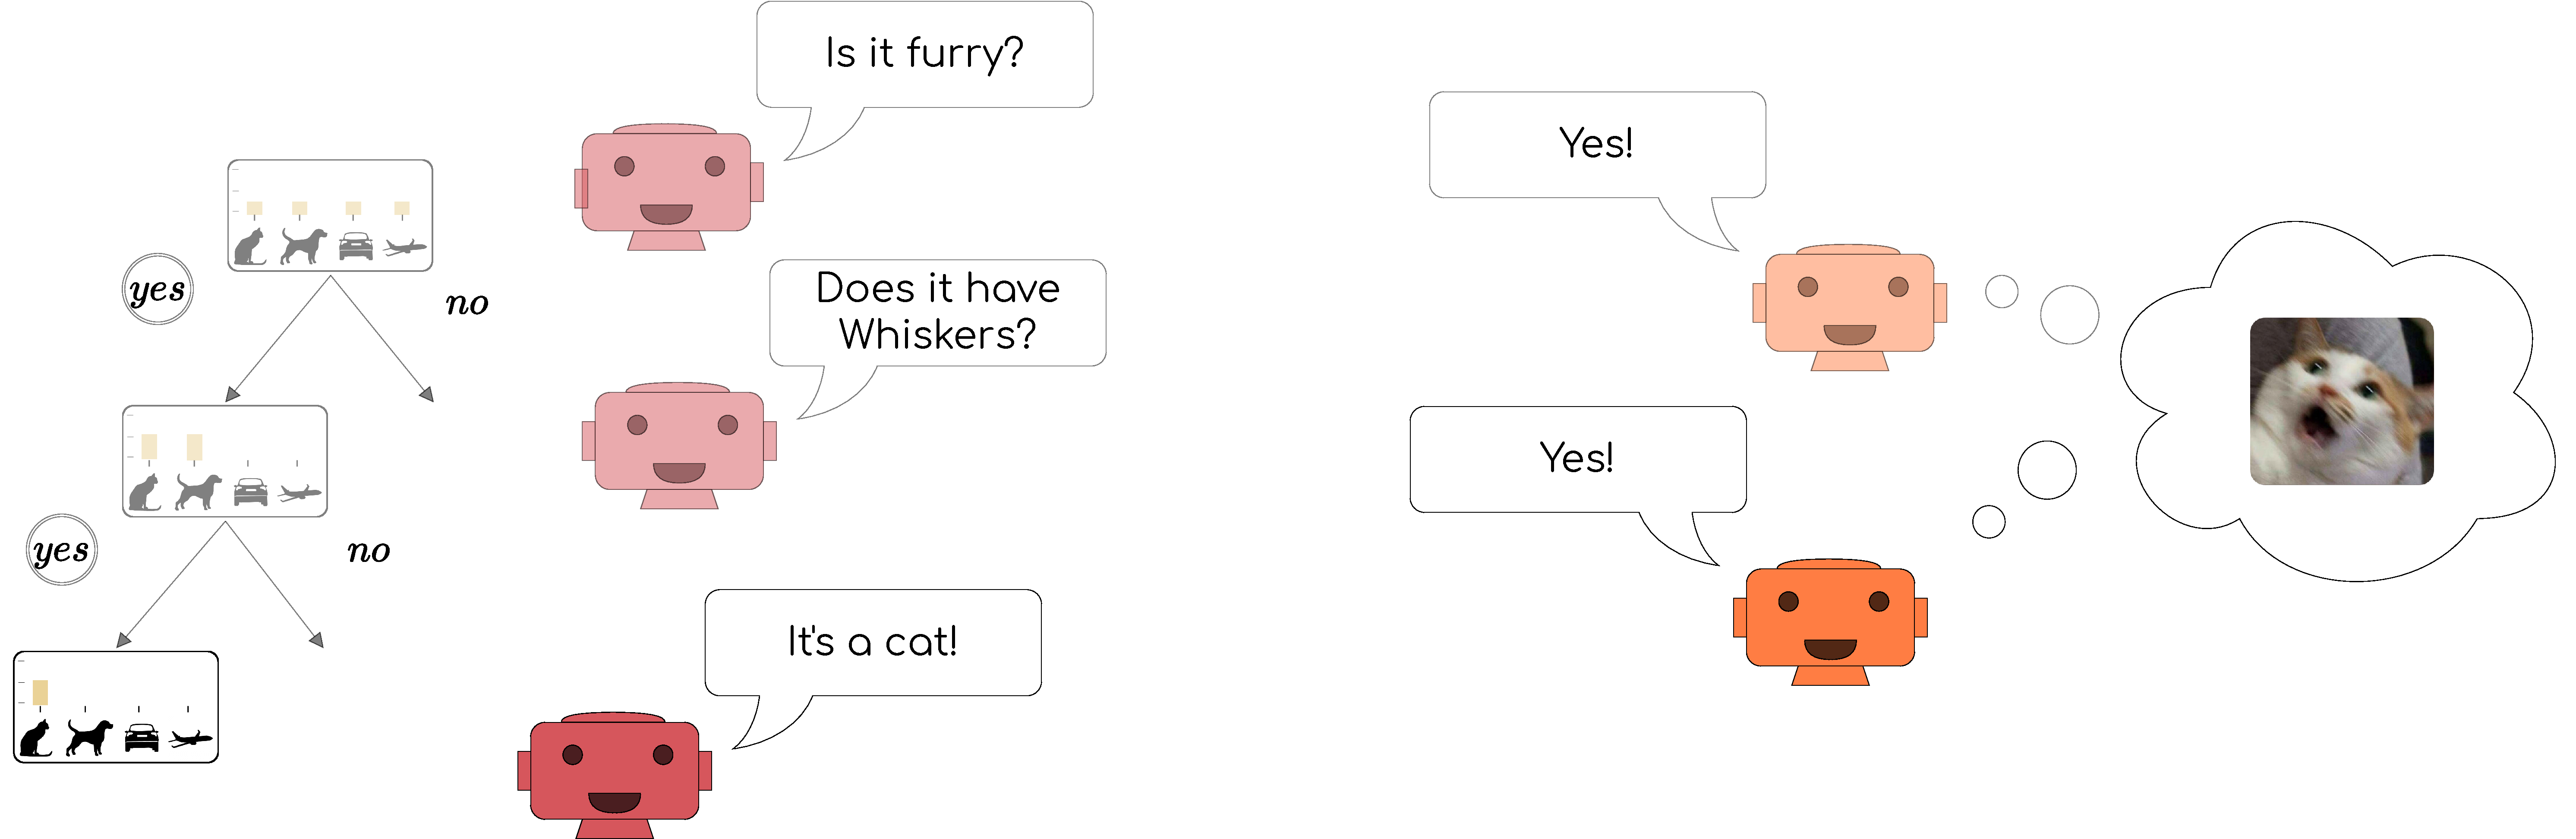
\includegraphics[width=0.7\textwidth]{images/rdtc_intuition.png}
	%\caption[caption for ]{After collecting images of birds, the ornithologist lets our proposed model classify the vast amount of data. Only in cases of high uncertainty, she is consulted and can classify the image manually. \footnotemark}
	%\label{fig:qual}
\end{figure}
\begin{itemize}\setlength\itemsep{1em}
	\item Two agents
	\item One is asking questions and one is answering them
	\item The unfolding decision process is an interpretable tree
\end{itemize}
\end{frame} 


\begin{frame}
\frametitle{What?}
\framesubtitle{Recap}
\begin{figure}
	\centering
	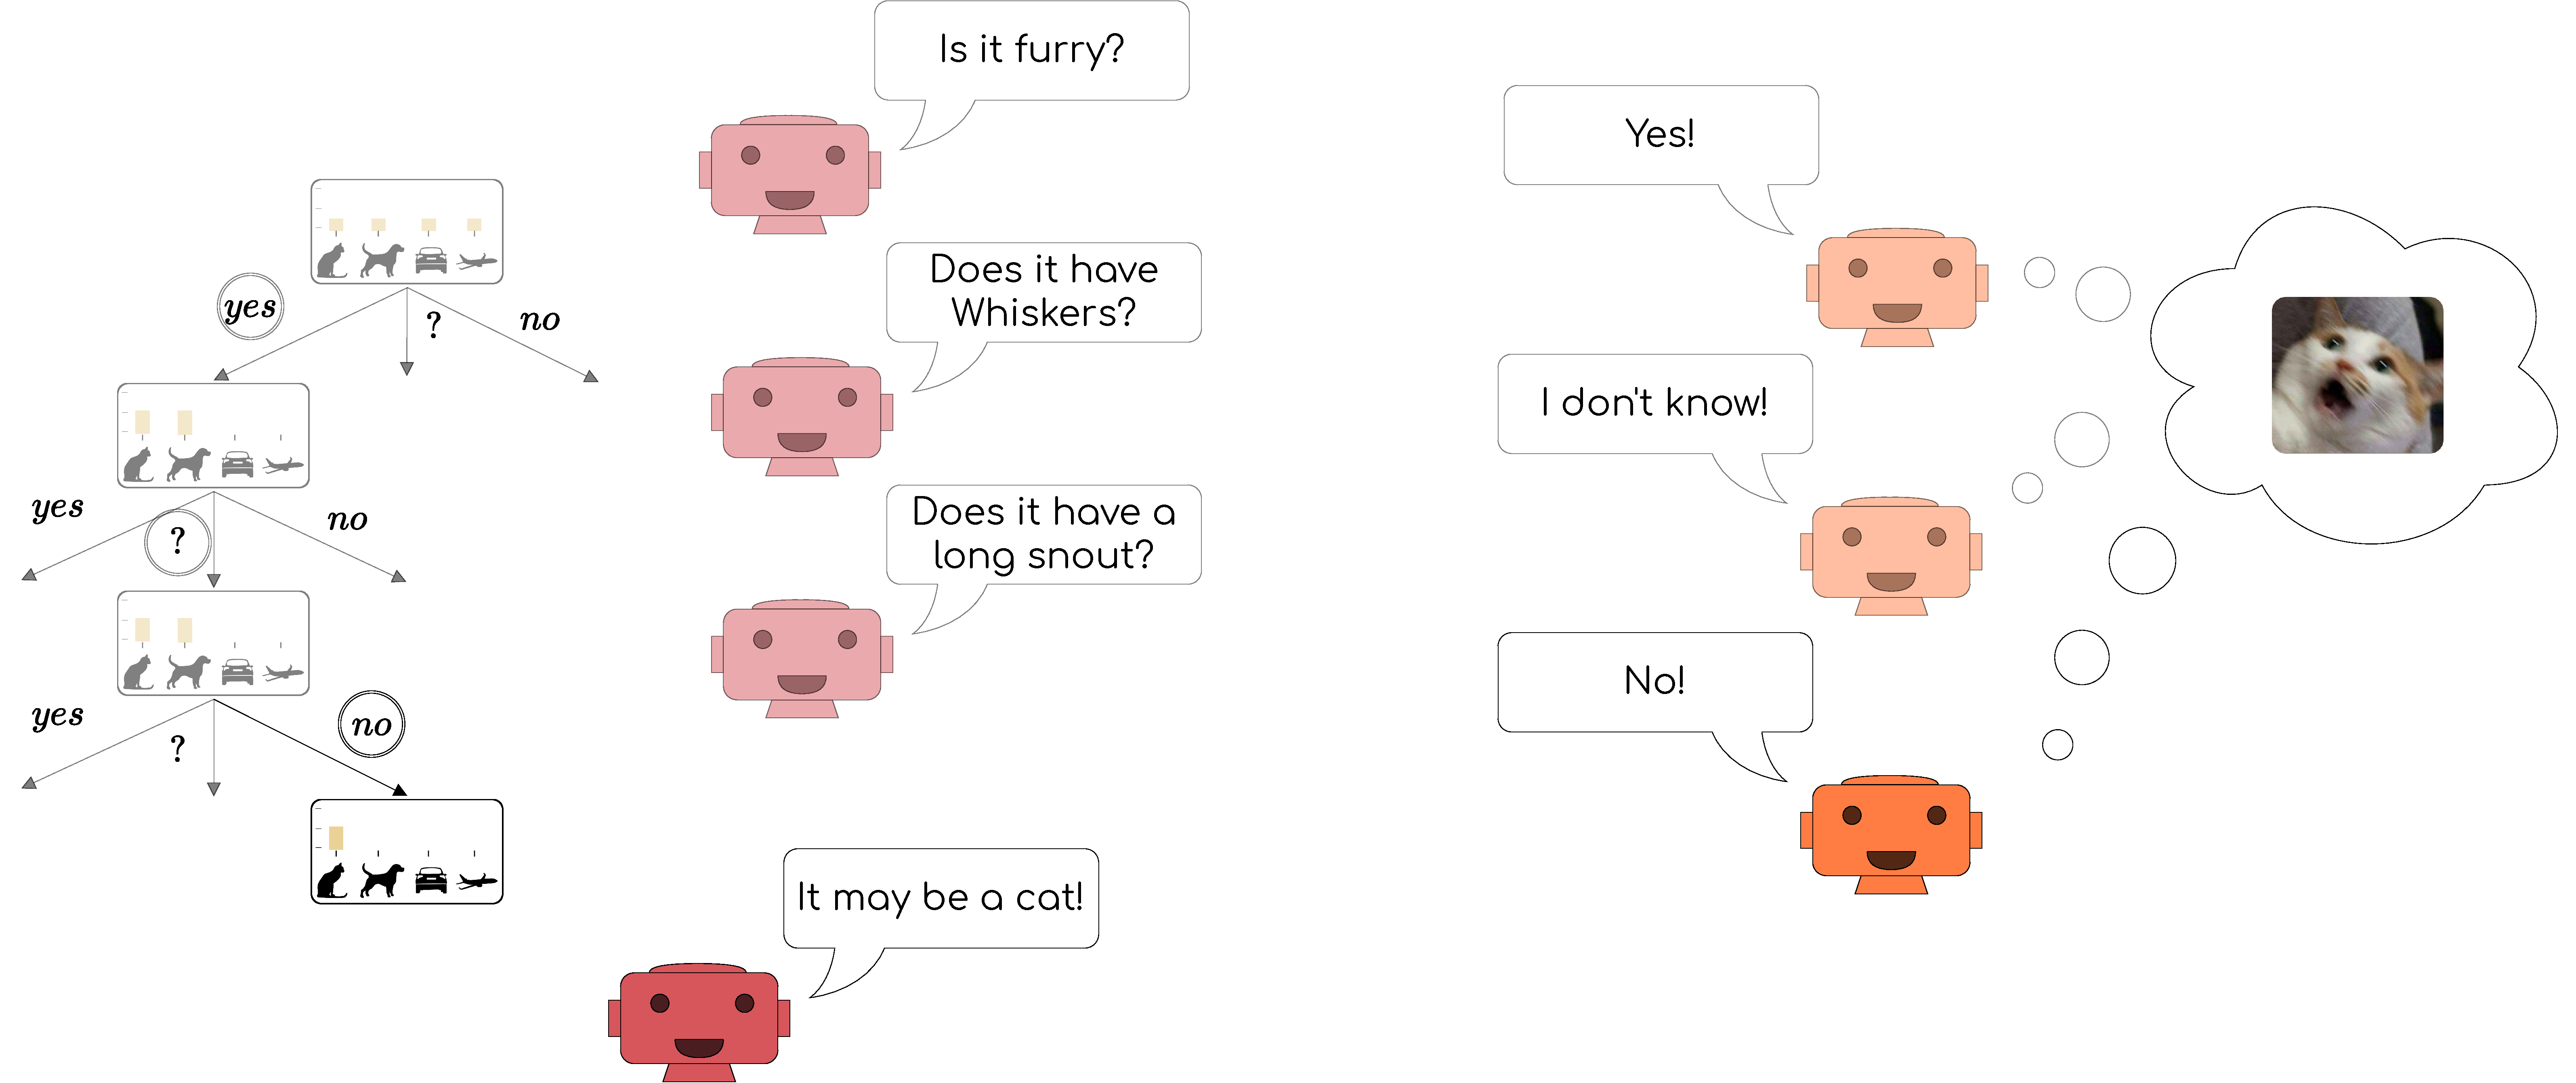
\includegraphics[width=0.9\textwidth]{images/urdtc_intuition.pdf}
	%\caption[caption for ]{After collecting images of birds, the ornithologist lets our proposed model classify the vast amount of data. Only in cases of high uncertainty, she is consulted and can classify the image manually. \footnotemark}
	%\label{fig:qual}
\end{figure}
\begin{itemize}\setlength\itemsep{1em}
	\item Two agents
	\item One is asking questions and one is answering them
	\item The unfolding decision process is an interpretable tree
\end{itemize}
\end{frame} 


%TODO simpler graphic here
\begin{frame}
\frametitle{What?}
\framesubtitle{Introducing Uncertainty}
\begin{figure}
	\centering
	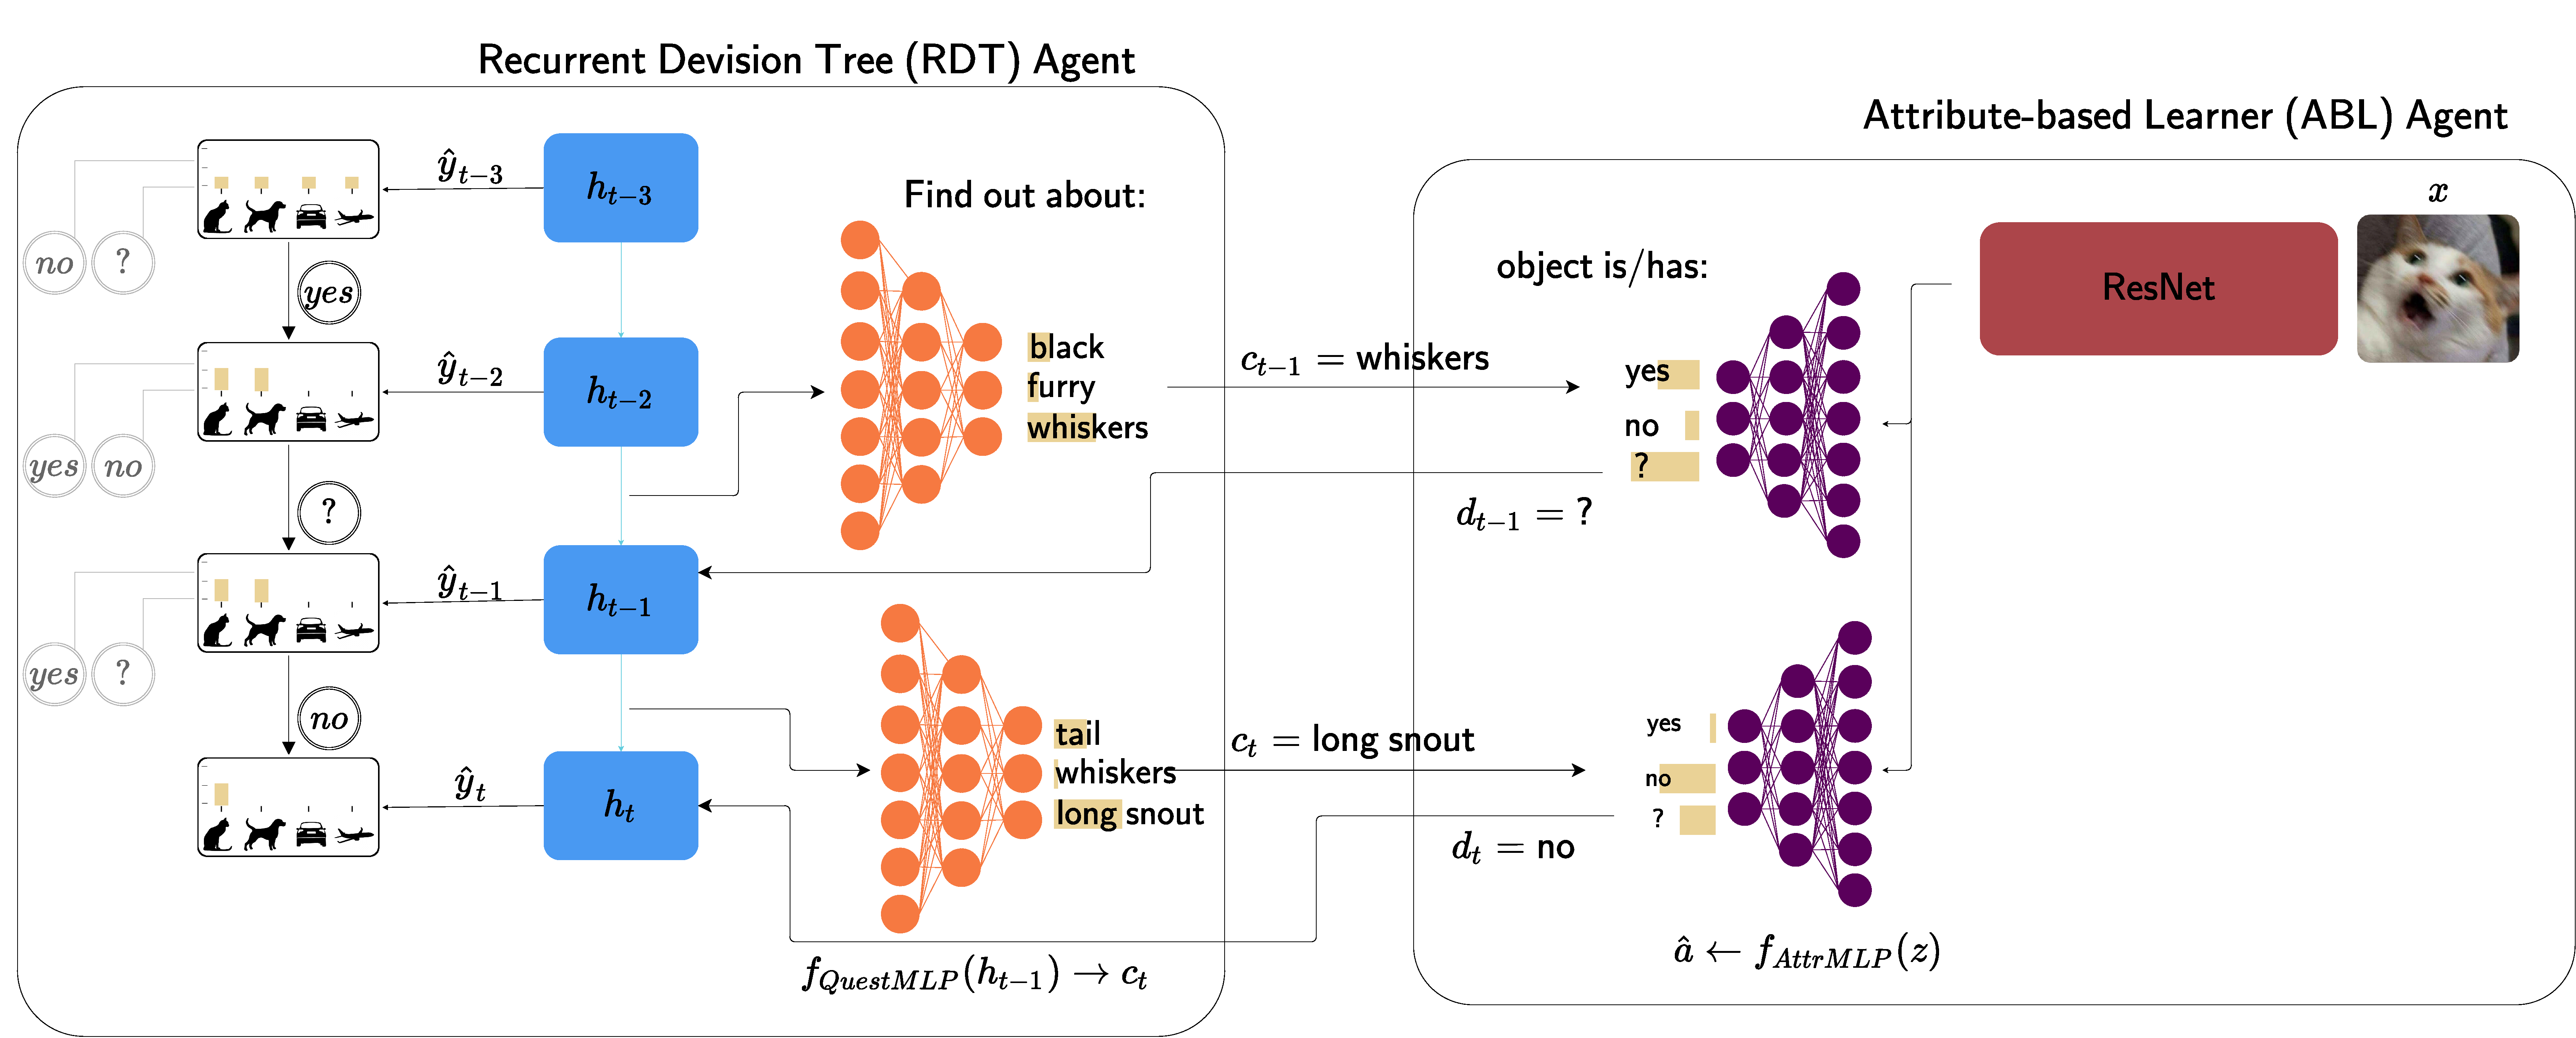
\includegraphics[width=1\textwidth]{images/uncertaintRDTC.pdf} 
	%\caption{The RDT asks questions about presence, absence or uncertainty of attributes. The answers, given by the AbL are used by the RDT agent to make a classification each iteration.}
	\label{fig:uncertainRDTC}
\end{figure}
\end{frame} 


\begin{frame}
\frametitle{Why do we need uncertainty?}
\framesubtitle{A Practical Example...}
	\begin{figure}
		\centering
		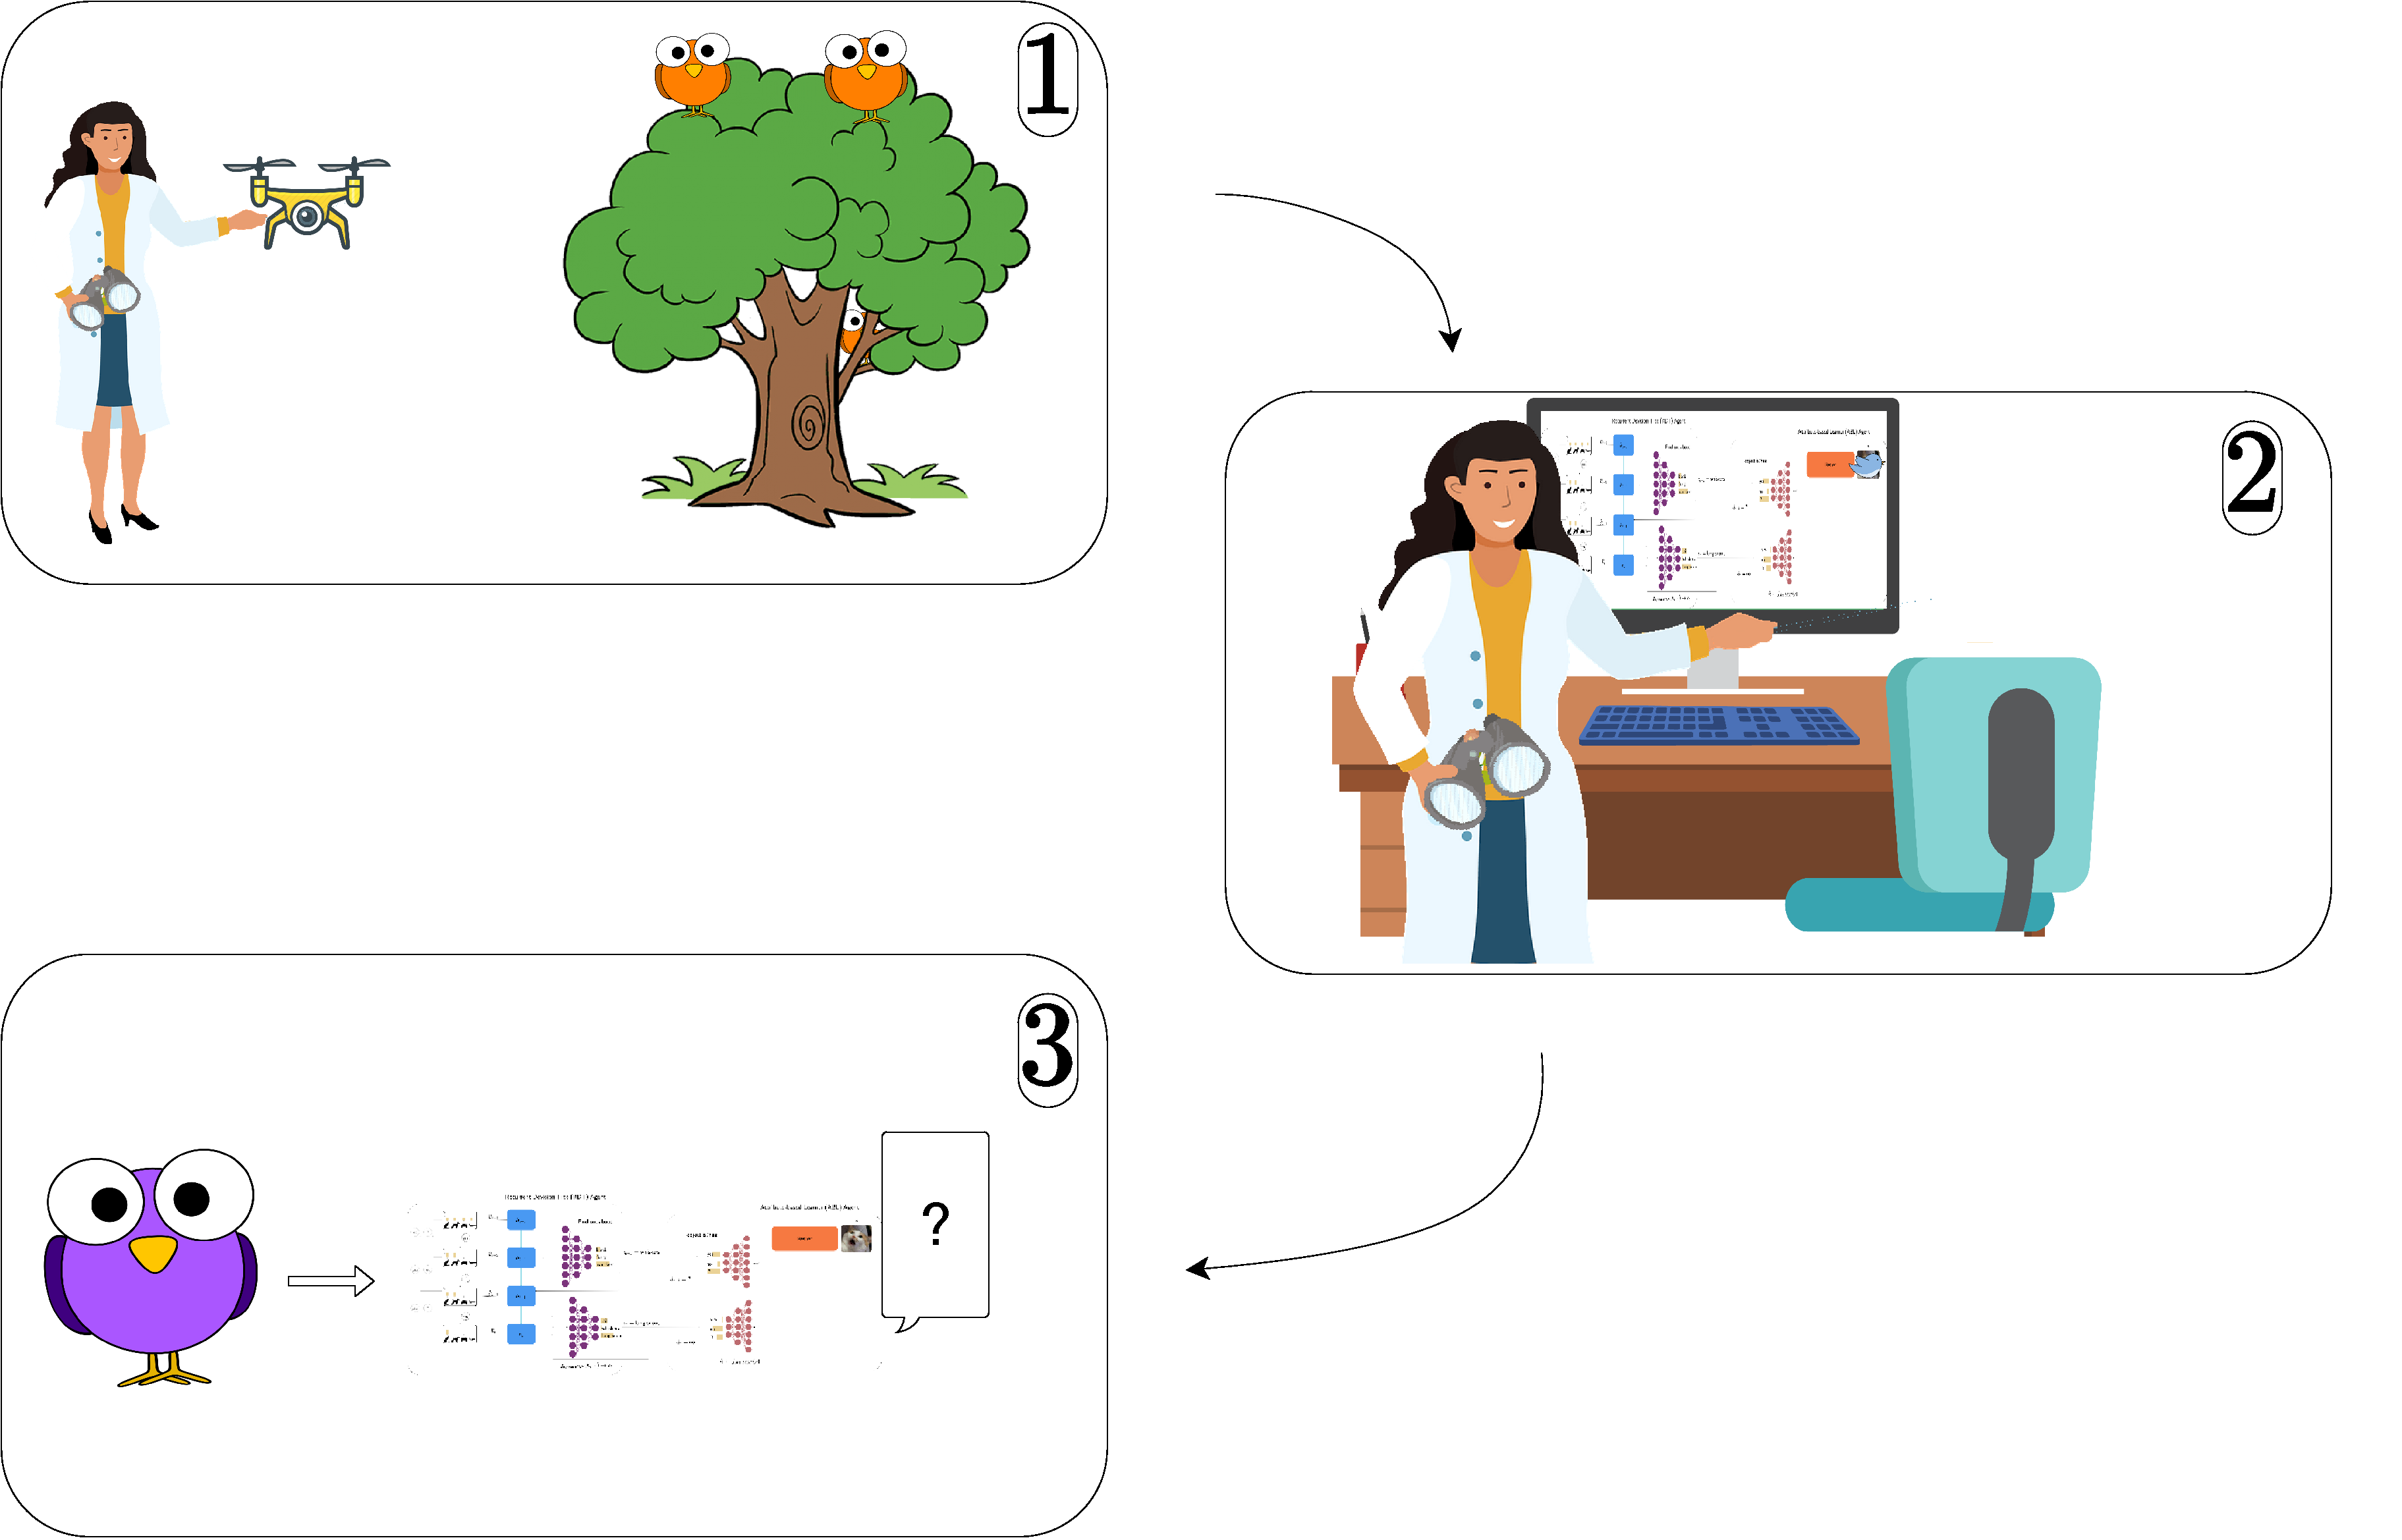
\includegraphics[width=0.6\textwidth]{images/ornithology.pdf}
		%\caption[caption for ]{After collecting images of birds, the ornithologist lets our proposed model classify the vast amount of data. Only in cases of high uncertainty, she is consulted and can classify the image manually. \footnotemark}
		%\label{fig:qual}
	\end{figure}
	\begin{itemize}\setlength\itemsep{1em}
	\item The ornithologist is tasked to survey bird species, which she automates using a drone and computer vision software
	\item She uses our model to go through the vast amount of collected data
	\item Some bird species unknown to the model appear in the data. The model yields high uncertainty and the ornithologist can classify them manually
	\end{itemize}
\end{frame}










% Related Work
\begin{frame}
\frametitle{Background}
\framesubtitle{Gaussian Processes (GP)}
\begin{figure}
	\centering
	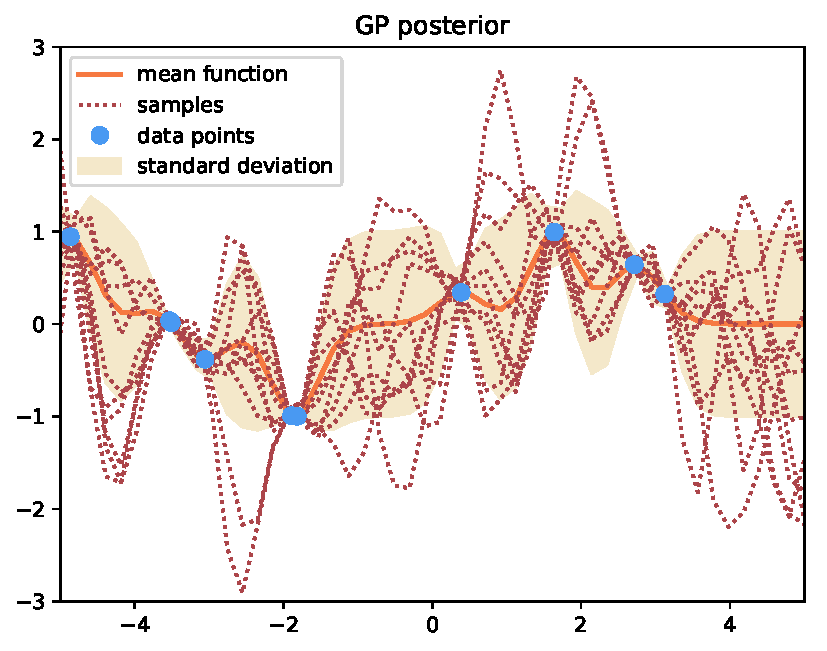
\includegraphics[width=0.4\textwidth]{images/post.pdf}
	\begin{itemize}
		\item Data points can be described by (infinitely) many functions
		\item A GP is a PDF over these functions
		\item Parameterized by mean function and covariance function
		\item The variance resembles the model uncertainty where no data is given
		\item 
	\end{itemize}
	%\caption{Correlations between misclassification rate, uncertainty, and usage of attributes.}
	%\label{fig:corr_matrix}
\end{figure}
\end{frame}




% Experiments
\begin{frame}
\frametitle{Experiments}
\framesubtitle{Investigating Uncertainties}
	\begin{figure}
		\centering
		
\includegraphics[width=0.6\textwidth]{images/corr_matrix.pdf}
		%\caption{Correlations between misclassification rate, uncertainty, and usage of attributes.}
		%\label{fig:corr_matrix}
	\end{figure}
\end{frame}



\begin{frame}
\frametitle{Experiments}
\framesubtitle{Investigating Uncertainties}
	\begin{figure}
		\centering
		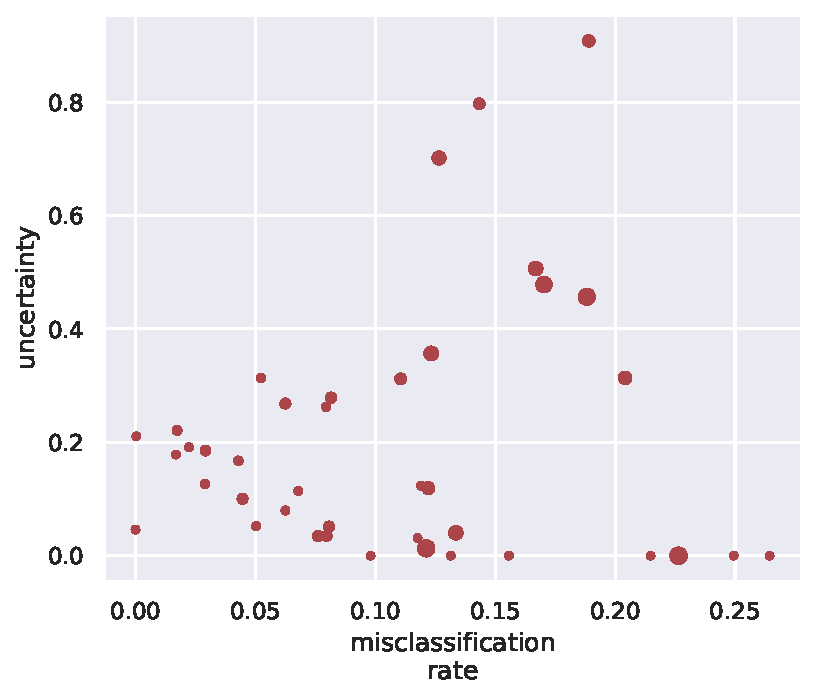
\includegraphics[width=0.6\textwidth]{images/error_sigma_corr_all.pdf} 
		%\caption{Misclassification rates of attributes and their respective uncertainties. The size of the points represents how often they are used.}
		%\label{fig:correlations}
	\end{figure}
\end{frame} 




\begin{frame}
\frametitle{Experiments}
\framesubtitle{OOD Detection}
\begin{figure}
	\centering
	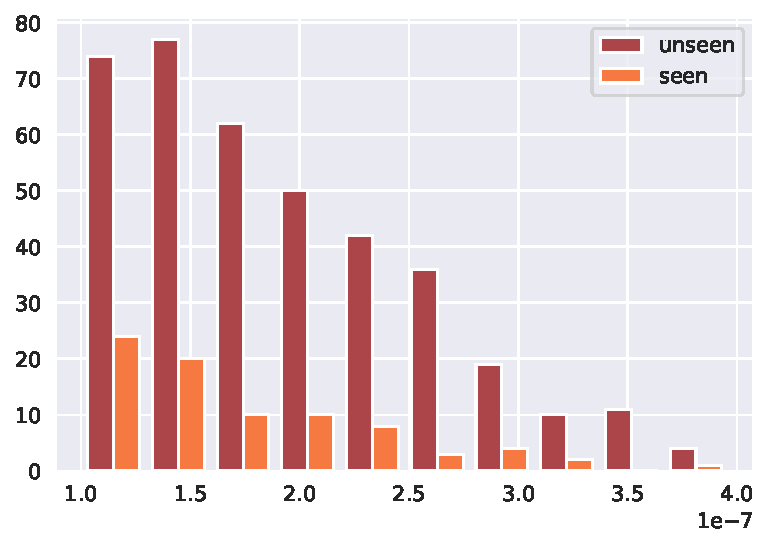
\includegraphics[width=0.6\textwidth]{images/zero_shot_class_uncertainty_median_hist.pdf}
	%\caption{Uncertainty values of attributes from seen and unseen classes. Examples from unseen classes have a higher attribute uncertainty. Attributes with an uncertainty value below $0.0000001$ are not shown.}
\end{figure}
\end{frame} 


\begin{frame}
\frametitle{Experiments}
\framesubtitle{Results on Benchmark Datasets}
\begin{table}
	\renewcommand{\arraystretch}{1.3}
	%\caption{We compare accuracy on AWA2, aPY, and CUB of our model and other methods. Standard deviations, denoted by $\pm$ are from five runs.}
	%\label{tab:benchmarks}
	\begin{tabular*}{\textwidth}{c @{\extracolsep{\fill}} c c c c}
		%\hline
		&                                AWA2&          aPY&          CUB\\
		\hline
		\hline
		ResNet \cite{he2016deep}&       98.2$\pm$ 0.0& 85.1$\pm$ 0.6 & 79.0$\pm$ 0.2 \\ 
		\hline 
		DT&                             78.0$\pm$ 0.4&64.3$\pm$ 0.6  & 19.3$\pm$ 0.3  \\ 
		\hline 
		dNDF\cite{kontschieder2015deep}&97.6$\pm$ 0.2&85.0$\pm$ 0.6 & 73.8$\pm$ 0.3 \\ 
		\hline 
		RDTC\cite{alaniz2019explainable}&98.0$\pm$ 0.1&85.7$\pm$ 0.7& 78.1$\pm$ 0.2   \\ 
		\hline 
		XDT&                            73.9$\pm$ 0.9&59.9$\pm$ 1.5  & 4.9$\pm$ 1.3 \\ 
		\hline 
		aRDTC\cite{alaniz2019explainable}&98.6&         86.1&  77.9$\pm$ 0.6\\ 
		\hline
		remRDTC(ours)&          98.7          &          86.4&  77.7\\ 
		\hline
		extRDTC(ours)&          98.7          &          85.4&  77.8\\
		%\hline 
	\end{tabular*}
\end{table}
\end{frame} 




\begin{frame}
\frametitle{Experiments}
\framesubtitle{Results on Benchmark Datasets}
\begin{table}
		\begin{tabular*}{\textwidth}{c  @{\extracolsep{\fill}}c c c c}
		& aRDTC \cite{alaniz2019explainable} & Random Baseline & remRDTC & extRDTC \\ 
		%\hline 
		%\hline
		\textbf{AWA2}& & & &\\\hline\hline
		Class &  98.6&  98.5&  98.7&  98.7\\ 
		\hline 
		Attribute & 80.4 & 84.6 &  87.5&  82.31\\ 
		&  &  &  &  \\
		\textbf{aPY}& & & &\\\hline\hline
		Class & 86.1&  86.5&  86.4&  85.4\\ 
		\hline 
		Attribute &  86.4&  86.2&  87.6& 87.12 \\ 
		&  &  &  &  \\ 
		\textbf{CUB}& & & &\\\hline\hline
		Class &  77.9& 76.8 & 77.7 & 77.8 \\ 
		\hline
		Attribute &  68.6&  70.0& 77.4 & 82.6 \\ 
		&  &  &  &  \\ 
	\end{tabular*}
\end{table}
\end{frame} 












% Conclusion
\begin{frame}
\frametitle{Conclusions}
\framesubtitle{A qualitative Example}
\begin{figure}
	\centering
	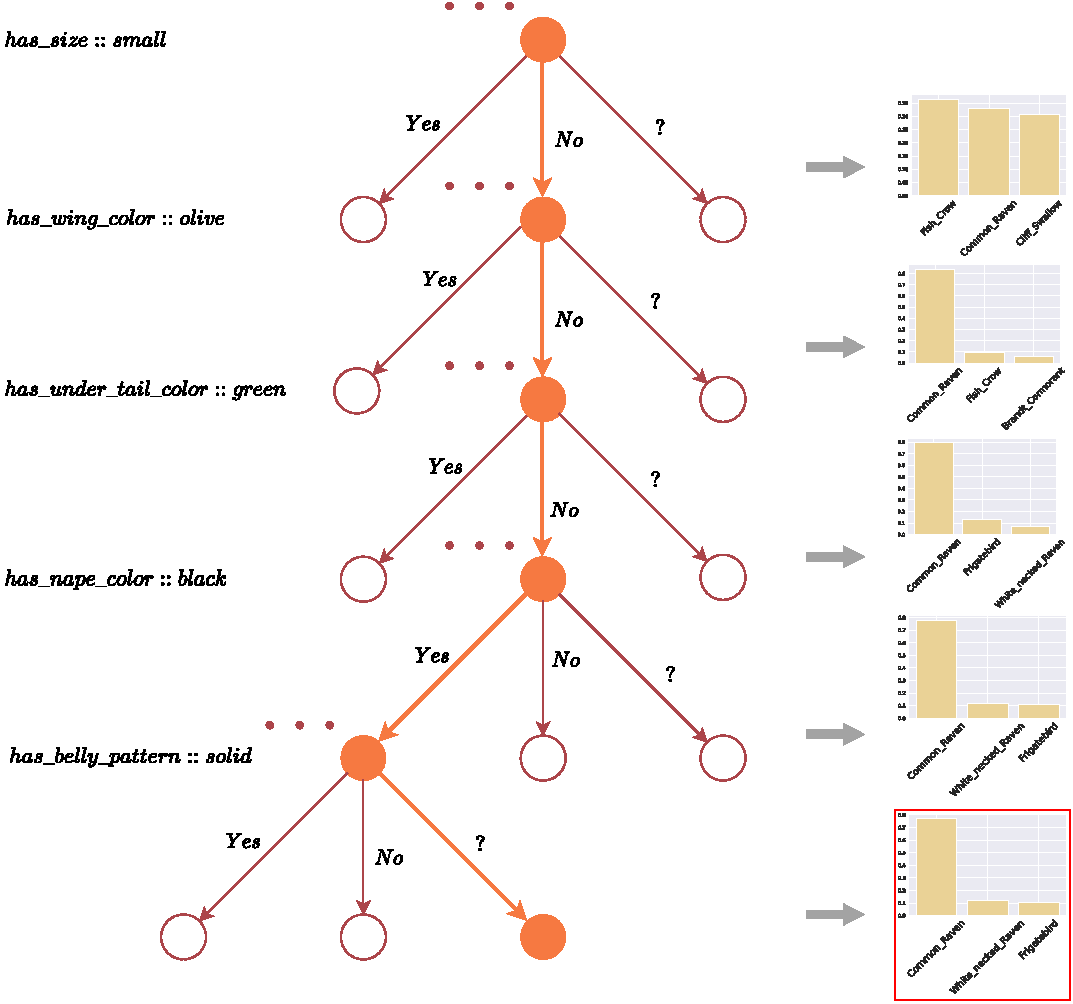
\includegraphics[width=0.7\textwidth]{images/example_tree.pdf}
%\caption{Five steps of a extRDTC decision process. The model has used an uncertain attribute and the final classification is wrong. In such a case, a human user could be consulted and manually classify the image. Note that the the softmax classification output is highly confident despite being wrong.}
\label{fig:example_tree}
\end{figure}
\end{frame} 

\begin{frame}
	\bibliographystyle{alpha}
	\bibliography{bibliography}
\end{frame}


\end{document}
